\chapter{Verteilungssicht}
Um eine Anwendung ausführen und betreiben zu können, ist ein gewisses Maß an Infrastruktur nötig. Da diese Infrastruktur besonders die querschnittlichen Konzepte beeinflusst, siehe Kapitel \ref{sec:quer} sei die für das Projekt eCourse benötigte Infrastruktur im Folgenden genauer beschreiben. \\

Für das Projekt eCourse gibt es im wesentlichen zwei Umgebungen auf denen das System läuft. Es gibt einen Aufbau beim Kunden auf dem dieses System läuft und es gibt den Aufbau zu Test- und Entwicklungszwecken. In Kapitel \ref{sec:Kunde}, wird kurz auf einen möglichen Aufbau der Infrastruktur beim Kunden eingegangen. In Kapitel \ref{sec:Entwicklung} wird auf den Aufbau der Infrastruktur zu Entwicklungs- und Testzwecken eingegangen.
\section{Infrastruktur beim Kunden}
\label{sec:Kunde}
Beim Kunden kann die Infrastruktur auf verschiedene Weise aufgebaut werden. In Abbildung \ref{fib:Kunde} ist ein möglicher Aufbau gezeigt. Die Qualität und Leistung dieser gezeigten Infrastruktur entspricht den geforderten Qualitätskriterien, daher wird sie vom Entwicklerteam empfohlen.

\begin{figure}[H]
\centering
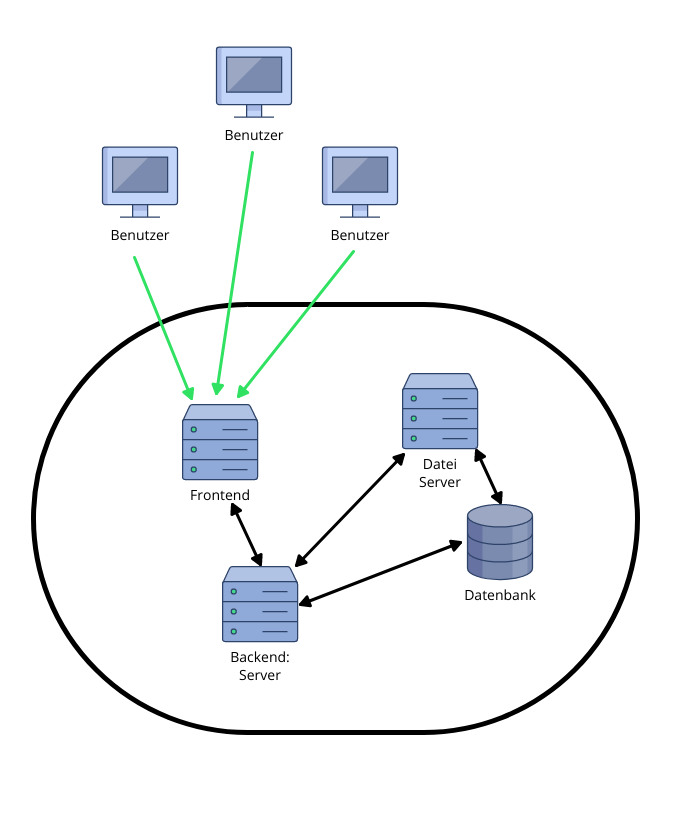
\includegraphics[height=0.8\textwidth]{kunde.png}
\caption{Mögliche Infrastruktur für eCourse beim Kunden}
\label{fib:Kunde}
\end{figure}


\section{Infrastruktur Entwicklung/Test}
\label{sec:Entwicklung}
Um die Anwendung zu entwickeln und zu testen wird vom Team die Infrastruktur in Abbildung \ref{fib:Entwickler} genutzt. Hierbei werden alle Komponenten auf einer Hardware realisiert. Dieser Aufbau dient vor allem dazu, dass die Entwickler zu jedem Zeitpunkt vollständigen Zugriff auf alle Komponenten des Systems haben. Ebenso wird dadurch die Zuverlässigkeit erhöht. Dadurch kann die Entwicklung beschleunigt werden.

\begin{figure}[H]
\centering
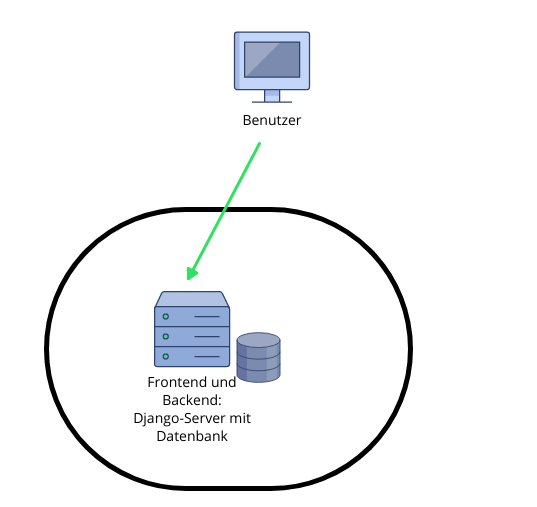
\includegraphics[height=0.6\textwidth]{entwickler.png}
\caption{Infrastruktur für eCourse zu Test- und Entwicklungszwecken}
\label{fib:Entwickler}
\end{figure}